\documentclass[12pt]{article}
\usepackage{listings,geometry,url}
\usepackage[dvipdfmx]{graphicx,color}
\geometry{a4paper}
\title{課題3}
\author{1029232337 杉本風斗}
\date{\today}
\begin{document}
\lstset{numbers=left,basicstyle=\small\ttfamily}
\maketitle
\section{Ex3.21}
示されたqueueの実装では,queueの先頭の要素へのポインタと末尾の要素へのポインタをペアとしてqueueのデータを表現しているため, あたかも2つ追加されているように見える.
\lstinputlisting{3-21.scm}
\section{Ex3.22}
記憶を頼りにがんばる.\\
\lstinputlisting{3-22.scm}
\section{Ex3.23}
リストの要素を(ひとつ前 . (要素 . ひとつ後ろ))というように表現し, queueと同じように先頭と末尾へのポインタのペアをdequeとする.\\
そうすると, 双方向に要素をたどることができるから示された操作をO(1)でできる.\\
要素が双方向にポインタを持っていることに注意して先頭・末尾への追加・削除の際にポインタを適切につなぎかえる.\\

\lstinputlisting{3-23.scm}
\section{Ex3.27}
\subsection{図}
ホワイトボードに書いたのをカメラで写したので割とひどい.\\
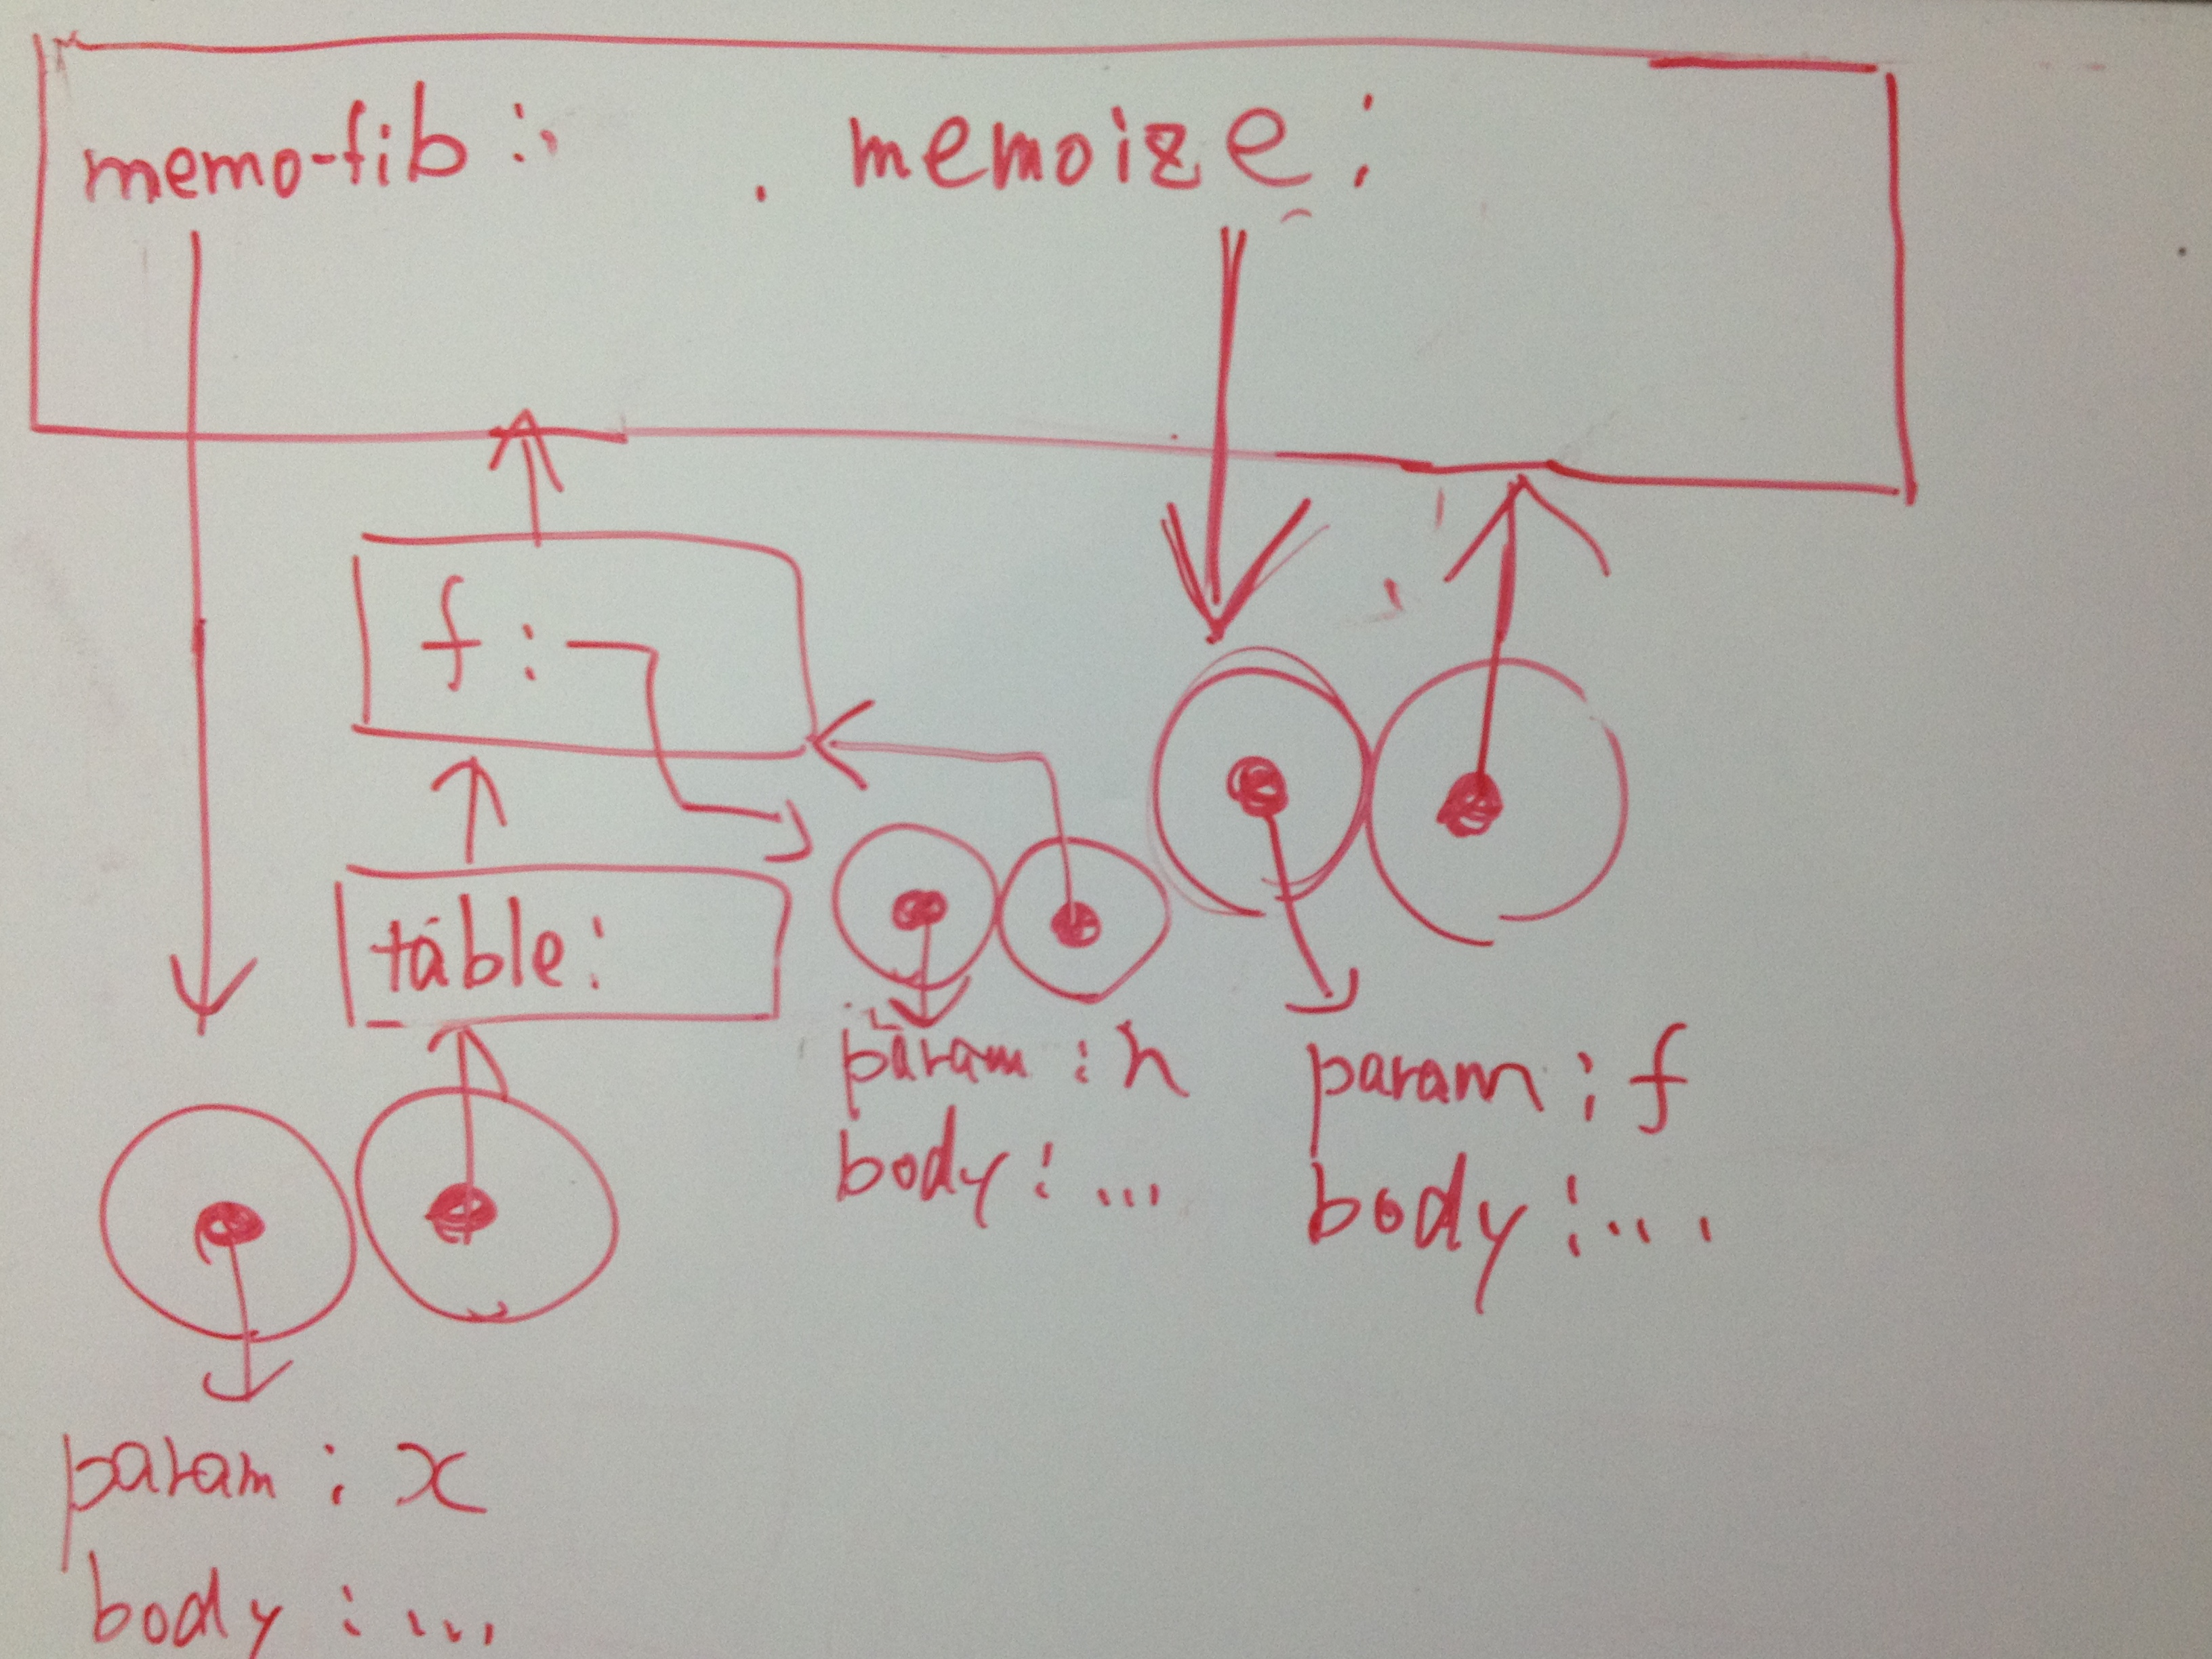
\includegraphics[width=10cm]{env.jpg}
\subsection{O(n)}
(memo-fib n)は, (memo-fib (- n 1))と(memo-fib (- n 2))を計算するが, (memo-fib (- n 1))で計算した結果がメモ化されるので(memo-fib (- n 2))は定数時間で計算できる.\\
よって, nに比例するステップ数で計算できる.\\

\subsection{(memoize fib)}
メモ化されていないfibが再帰的に呼び出されるためうまく計算時間を抑えられない.\\

\end{document}
